\section{System Design}\label{sec:design}

\begin{figure}[t]
\centering
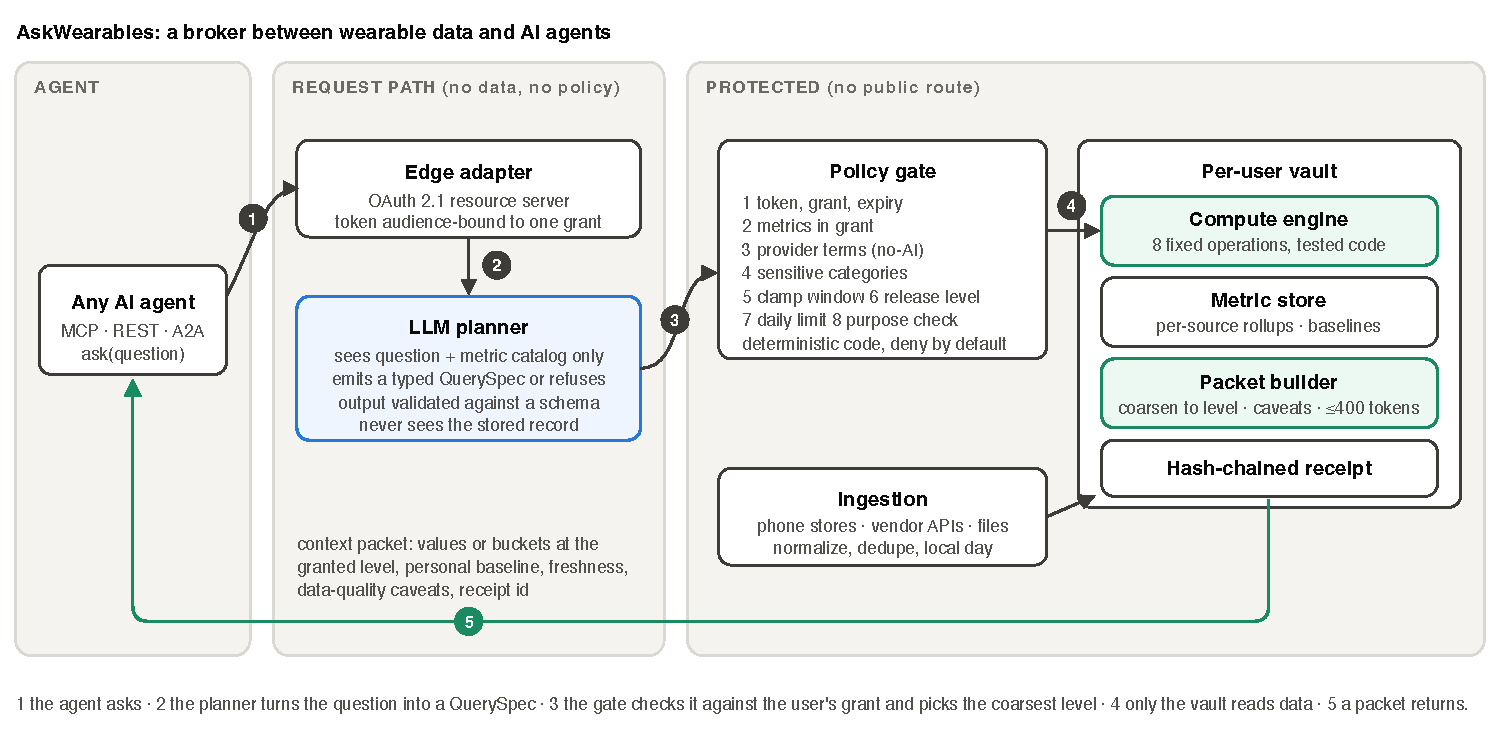
\includegraphics[width=\textwidth]{figures/fig_architecture.pdf}
\caption{Request flow. The agent sends a question (1); the planner turns it into a QuerySpec without seeing any
data (2); the gate checks the QuerySpec against the user's grant and picks the coarsest release level (3, step 7 in
the gate box is the daily release limit, ``daily budget'' in the figure); only the per-user vault reads health data, computes the answer and
builds the packet (4); the packet and a receipt identifier return to the agent (5). Seven Cloudflare Workers form
four trust zones: public (site, console), identity (auth), request path (edge, planner) and protected (gate,
vault). The planner and the edge hold no binding to data or policy, and a test checks the bindings between
Workers.}
\label{fig:arch}
\end{figure}

\sys{} separates three decisions that the prevailing designs leave to the agent model: what to compute, what to
release, and how to say it. \Cref{fig:arch} shows the request path. We describe the components in the order a
question meets them after ingestion: the metric layer that defines every number (\cref{sec:metric}), the planner
(\cref{sec:planner}), the gate (\cref{sec:gate}) and the packet and receipt (\cref{sec:packet}).

\subsection{Data model and metric layer}\label{sec:metric}

\paragraph{Records.} Every value is stored with its source, method and device. Timestamps are stored in UTC with
the original offset, so that a \emph{day} is the user's local day at the time of the sample and travel does not
split a night. Sleep is attributed to the wake date. Upserts are idempotent on the pair (source, external
identifier), so a repeated sync never double-counts.

\paragraph{One source per metric and day.} When two devices report one metric on the same day, the metric layer
picks one source rather than summing them: first a source with valid coverage, then by device class (watch, ring,
band, scale, glucose monitor, phone). Steps are never summed across sources.

\paragraph{Coverage.} Intraday metrics count the hours with data against 12 expected hours (steps, active energy)
or 16 (heart rate); nightly and vendor-daily values count a day as covered. A day under 60\% coverage is marked as
low-coverage and excluded from baselines. Gaps are never interpolated.

\paragraph{Personal baseline.} A personal baseline is the median and interquartile range (IQR) of the trailing 28
valid days of the same source, and needs at least 14 such days. Because it is computed per source, it restarts
when the user changes device. A value inside the IQR is \emph{within usual}; outside it, the distance to the
nearer quartile, in units of the IQR, places it \emph{slightly} (up to 0.5), \emph{moderately} (up to 1.5) or
\emph{far} above or below usual. Proprietary vendor scores (readiness, recovery, strain) are kept apart and never
merged.

\paragraph{Catalogue.} The catalogue defines 15 metrics, each with one unit, one daily aggregation and a plausible
physical range checked on ingest. Four sensitive categories (blood glucose, cycle tracking, ECG and rhythm
notifications, sleep-apnea events) are listed only so that the gate can refuse them by name.

\paragraph{Operations.} The compute engine offers eight operations: \code{latest}, \code{aggregate} (total, mean,
minimum or maximum), \code{trend} (an ordinary least-squares slope, reported only when $|t|\geq 2.5$),
\code{compare\_to\_baseline}, \code{compare\_periods}, \code{threshold\_check} (days meeting a condition),
\code{correlate} (Spearman's rank correlation, with an optional lag) and \code{list\_sessions}. Medians, spreads,
percentages, heart-rate zones, per-workout metrics and queries whose window depends on another query are
deliberately not offered.

\subsection{Planner}\label{sec:planner}

The planner is a language model that emits a JSON object, validated in code against the QuerySpec schema; the
deployed service also requests schema-constrained decoding from the model provider. Its prompt holds the date, the user's time zone, the
metric catalogue, the eight operations, rules for resolving relative windows and a list of question types to
refuse; it never holds data. The question is passed as data, truncated to 500 characters, with an instruction to
ignore any request inside it. The model either emits a QuerySpec, which names the metrics, the operation, the
window and the operation's parameters, or refuses.

The model's output is validated against the QuerySpec schema in code. A spec that fails validation is retried once
on a second model and then refused. In the study, a keyword pre-check refused questions that named a sensitive category before
any model was called; it has since been removed, since the prompt refuses those categories and a plan naming a
sensitive metric is refused in code (all 20 sensitive questions and none of 10 near-misses refused without it;
\code{eval/scripts/planner-sensitive.ts}). The planner runs at temperature 0. The deployed primary model is \code{llama-3.3-70b} with
\code{gpt-oss-120b} as the second model, chosen by the measurement in \cref{sec:res:planner}. During the study a keyword-rule planner was a last fallback when both models were
unreachable; it has since been removed, so the deployed service refuses such a request as \emph{planner unavailable},
and the owner's console plans its own questions through the same planner.

\subsection{Policy gate}\label{sec:gate}

The gate is plain code that runs before any data is read and denies by default. It applies, in order:
\begin{enumerate}[leftmargin=1.6em,itemsep=1pt]
\item a valid token bound to this agent, and a grant for the same agent and user that has neither expired nor been
  revoked;
\item every requested metric in the grant;
\item provider terms flags: data from a source whose terms forbid AI use never reaches a model-facing agent;
\item sensitive categories only when the grant names them one by one;
\item the window clamped to the grant's maximum window, ending no later than today;
\item the release level set to the lower of the grant's maximum and the lowest level that answers the operation;
\item the daily release limit: the number of packets already released to this agent today (not exercised in this
  study, where the limit was set far above any run's needs);
\item a contextual-integrity check of the grant's purpose against each metric's category and the level, which can
  lower the level or deny, but never raise it;
\item a receipt, written for releases and denials alike.
\end{enumerate}

\paragraph{Purpose.} A grant names one of five purposes (scheduling, training advice, sleep coaching, general
wellness, personal research). Each purpose permits a set of metric categories and a maximum level; for example, a
scheduling grant permits sleep, heart and activity metrics at level 1 at most. The purpose is fixed in the grant at
consent time. An agent cannot restate it in a request: a purpose argument in a request is recorded and ignored.

\paragraph{Coarsen rather than deny.} When the grant's maximum level is below the lowest level an operation needs,
the gate releases the coarser level instead of denying. A request for the latest value at level 1, for example,
returns \emph{within} or \emph{below usual} without a number. Denying would push agents to retry with other
phrasings.

\subsection{Packets and receipts}\label{sec:packet}

\paragraph{Release levels.} A packet holds only its level's view of each finding:
\begin{itemize}[leftmargin=1.4em,itemsep=1pt]
\item level 0, \emph{flag}: for example, a threshold was or was not met;
\item level 1, \emph{bucket}: a direction and a magnitude bucket against the user's baseline;
\item level 2, \emph{values}: values with units, including daily values;
\item level 3, \emph{raw}: raw samples and session detail.
\end{itemize}
Each operation has a lowest level that can answer it: \code{threshold\_check} needs level 0; \code{trend},
\code{compare\_to\_baseline}, \code{compare\_periods} and \code{correlate} need level 1; \code{latest},
\code{aggregate} and \code{list\_sessions} need level 2. The gate releases that level unless the grant or the
purpose caps it lower. A threshold question about sleep therefore returns a flag and a count of days, not the
nightly durations. This is the broker as studied; in the broker as deployed, after the two steps of
\cref{sec:v2-design}, a threshold check that asks how many days met a condition is released at level~1, which
carries the count, and a denial names a closely related granted metric where there is one.
Free text from providers, such as workout titles and notes, appears only at level 3. Every packet also carries a
data-quality block (freshness, coverage, sources, baseline length and caveats such as a device change or a
time-zone change in the window), the data version, and a flag stating that it is not medical advice. Packets at
levels 0 to 2 are held to at most 400 tokens by dropping the oldest daily values first.

\paragraph{Determinism.} Each packet carries a \emph{data version}, a hash of the user's stored data, and an
\emph{as-of} time rounded down to the hour. The same QuerySpec at the same level, data version and as-of hour returns a
byte-identical packet; the receipt identifier travels outside the packet for this reason.

\paragraph{Example.} The QuerySpec for ``How many steps did I take in total over the last 7 days, ending
yesterday?'' asked on 2026-11-25 is
\begin{quote}\small
\code{\{"metrics":["steps"], "operation":"aggregate",}\\
\code{\ "window":\{"start":"2026-11-18", "end":"2026-11-24"\},}\\
\code{\ "params":\{"statistic":"total"\}\}}
\end{quote}
For the person with missing days, its level-2 packet states the total of the
recorded days, says that only 4 of 7 days are covered, adds the caveat ``3 of 7 days have no steps data'', and
lists the four daily values (\cref{tab:examples}).

\paragraph{Receipts.} Receipts are append-only and hash-chained per user, and the chain head is anchored daily in
object storage. A receipt records the agent, grant, purpose, decision, level, metrics, window, QuerySpec, packet
hash and the gate's reasons. Receipt payloads are encrypted with a per-user data key. Deleting a user destroys that
key, which erases the payloads while keeping the chain verifiable.
